%related work
%references and citations
%从头到尾读一遍
%把代码里的cmu.symonster去掉
\documentclass[twocolumn]{article}
\usepackage{typearea}
\paperwidth 8.5in \paperheight 11in
\typearea{15}
\usepackage{latexsym,graphicx}
\usepackage{amsmath,amssymb,enumerate}
\usepackage{amsthm}
\usepackage{xspace}
%\usepackage[showonlyrefs,showmanualtags]{mathtools}
\usepackage{bm}
\usepackage{ifpdf}
\usepackage{shadow,shadethm,color}
\usepackage[compact]{titlesec}
\usepackage{algorithm}
\usepackage[noend]{algpseudocode}
\usepackage{float}
%\numberwithin{algorithm}{section}
\usepackage{subfigure}
\usepackage{verbatim}
%\usepackage{times}
\usepackage{paralist}
\usepackage{enumerate}
\usepackage{changepage}
\setlength{\parindent}{0pt}
\title{Type Activation Approach to Component Based Program Synthesis}
\author{Kaige Liu, Tianlei Pan}
\date{}
\begin{document}
\maketitle
\section*{Abstract}
Component based program synthesis generates programs consisting of a set of given components. In this paper, we present a new type activation algorithm for component based synthesis. Our approach builds a network structure to model program components, and generate possible code snippets by finding reachable paths on the network. The target program generated by our algorithm is guaranteed to compile and pass all test cases provided by the user. We also explored an optimization technique in Component based program synthesis that uses interprocedural analysis to eliminate equivalent program to improve performance of our approach.\\

We have implemented this algorithm with a tool called SyChicken[6], which synthesizes Java code from Java APIs. We have tested SyChicken against various benchmarks, and proved that it is able to synthesize real-world programming tasks. In terms of performance, we compared SyChicken against SyPet[3], a state-of-the-art approach, and demonstrate advantages in encoding complexity of SyChicken against SyPet.\\


\textit{Keywords}: type activation, program synthesis, component based, interprocedural analysis.\\


\section{Introduction}
Component based program synthesis generates programs consisting of a set of given components. Nowadays, as software libraries grow, it becomes more and more difficult for programmers to learn and find the right method that satisfies certain specification. A program synthesis tool can save their time by automating the API finding process.\\

In this research, we will focus on a type-oriented program synthesis. User will specify the signature of the target program, including input and output types, and provide test cases. Our algorithm will search for the target program which satisfies all given constraints.

\subsection{Sypet}
SyPet[3] is a state-of-the-art component based synthesis tool that adopts a modified graph representation called Petri-Net and by using nodes, edges and tokens to represent types, methods, and variable constraints. Tokens are initially given to each input types. Each method call will “fire” tokens from its input types to return type to represent variable consumption and production. A reachable path is defined as a sequence of method calls, which consume all tokens in all types but the return type, which correspond to a viable program synthesis solution. To find a reachable path, the reachability analysis is modeled as a Boolean satisfiability problem. SyPet is able to synthesize a large variety of code snippets coming from a wide range of real world libraries such as java.awt.geom, joda, jsoup and apache math. However, we identified the following problems of SyPet. Firstly, to model the reachability analysis as token firing with time sequence, a Boolean variable is created for each method on each possible time step, which creates an overhead for the SAT model. Secondly, the notion of token firing means that a variable will be consumed once it’s used in the program, which is not always true in modern programming languages. To deal with this problem, SyPet allows each type to be “cloned”, adding a transition for each type to directly produce one additional token for a type. For the reachability analysis, cloning a variable is equivalent to increasing the program length by 1, which also enlarge the space of reachable paths.
\subsection{Motivating example}
An example task is given below:
\begin{itemize}
    \item Example signature: Given input MyPoint, output Point.
    \item Example library name: Point.jar.
    \item Example test cases: specified in Figure 1.
    \item Target solution: Figure 2.
\end{itemize}
\begin{figure}[h]
\centering
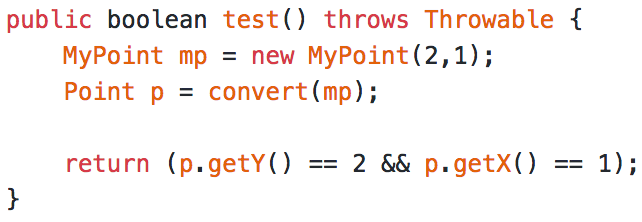
\includegraphics[scale = 0.65]{testcase.png}
\caption{Example test case}
\end{figure}

\begin{figure}[h]
\centering
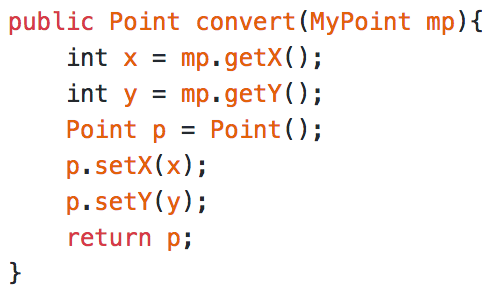
\includegraphics[scale = 0.65]{sample_solution.png}
\caption{Example solution}
\end{figure}
\subsection{Hypothesis}
We make the following assumptions on our target program:
\begin{itemize}
    \item The program is a straight line program with no conditional or loop.
    \item Each line of the program correspond to exactly one call in the specified program components.
    \item Each return value is used at least once.
\end{itemize}
\begin{figure*}
\centering
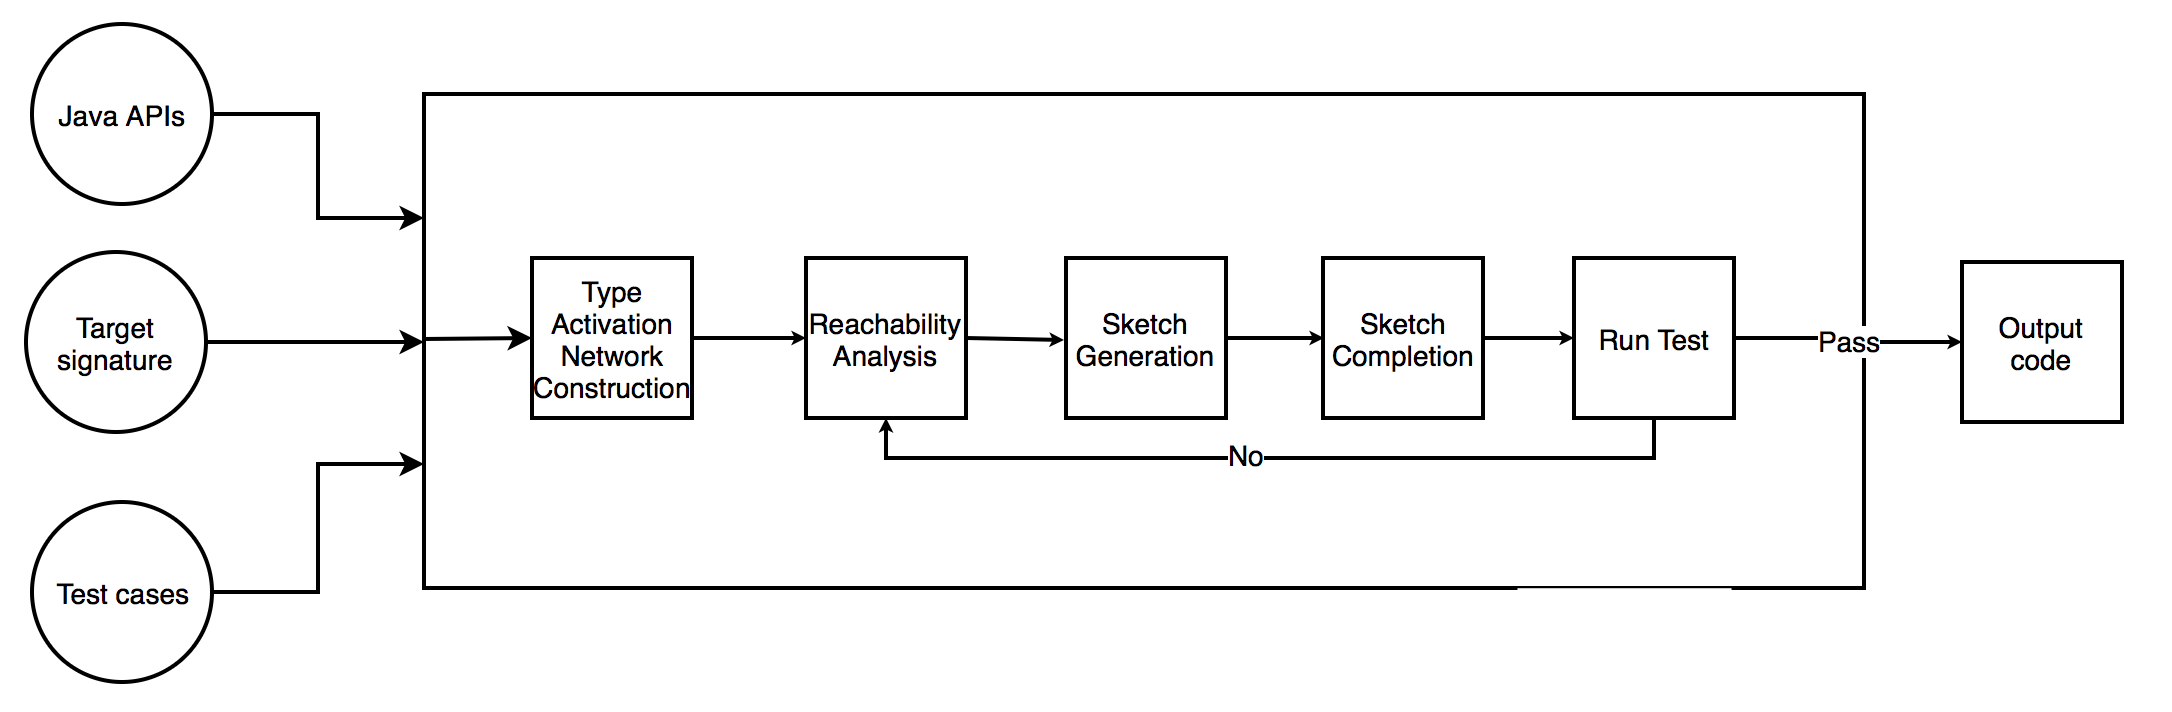
\includegraphics[width=\textwidth]{overviewhor.png}
\caption{Algorithm Overview}
\end{figure*}
\section{Algorithm Overview}
In this section we aim to give an overview of our synthesis algorithm, and demonstrate our algorithm with the example from. A brief overview over the algorithm is shown in Figure 5. Our algorithm takes a method signature $S$, a set of components $\Wedge$, and test cases $E$. Its output is either $\bot$, meaning that the specification cannot be synthesized using components $\Wedge$, or a program that compiles and passes all test cases $E$.\\
\subsection{Network Construction}
Similar to SyPet, our algorithm first constructs a network $N$ to model the provided components. In the network, we model each method and each type as nodes. A certain method and a type are connected with an edge when a method uses a certain type as input/return type. Each vertex in the network can be activated, meaning the type/method appears in the target program. An example network is shown is Figure 4.\\
\begin{figure}[H]
\centering
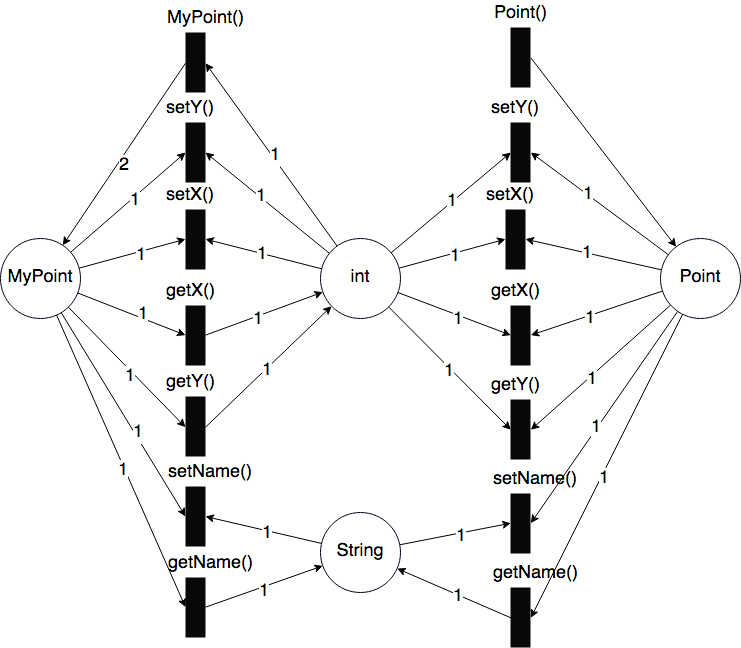
\includegraphics[scale = 0.3]{point.png}
\caption{A generated network for Point.jar}
\end{figure}
\subsection{Reachability Analysis}
The second part of our algorithm is reachability analysis. A reachable path on network $N$ is defined as a set of methods that satisfy constraints, which we will specify later. Reachable paths are found with a SAT solver.\\ 
\subsection{Sketch generation}
Next we generate program sketches from each reachable path. A program sketch is a ordered sequence of program components. To generate sketches, we basically add order to the set we found in reachability analysis.\\
\subsection{Sketch completion}
The fourth part of our algorithm is sketch completion. To generate code from program sketches, we need to determine which variables are used as input to each input. Our technique uses a SAT solver to find possible completions of the generated program sketch.\\

\section{Network construction}
As we mentioned before, the network $N$ models the given program components. Our network $N$ is a bipartite multigraph with 2 types of nodes: types, drawn as circles and methods drawn as rectangles. We define our network $N = (T,M,E,A)$ by
\begin{itemize}
    \item $T$ is the set of all possible types in the program components.
    \item $M$ is the set of all possible methods in the program components.
    \item $E \subseteq (T\times M \times \mathbb{N})\cup(M\times T \times \mathbb{N})$ such that $(t,m,i) \in E$ if and only if method m requires type t as its input, and $(m,t,i) \in E$ if and only if method m returns type t. If one type takes in multiple inputs of the same type, multiple edges will be added to E.\\
\end{itemize}

One important variation to handle in object-oriented programming languages is polymorphism of types. To handle polymorphism, in addition to the original set of methods, we add an additional transition from any subclass to its super class, therefore any subclass can be considered as its super class by an additional transition.\\

Each node in the network can be activated, defined in the activation set $A \subseteq M\cup T$. Activation of each type/method encodes the information whether the type/variable is in the target program, and the set A will be found by the reachability analysis process.

\section{Reachability analysis}
\begin{figure}[h]
\centering
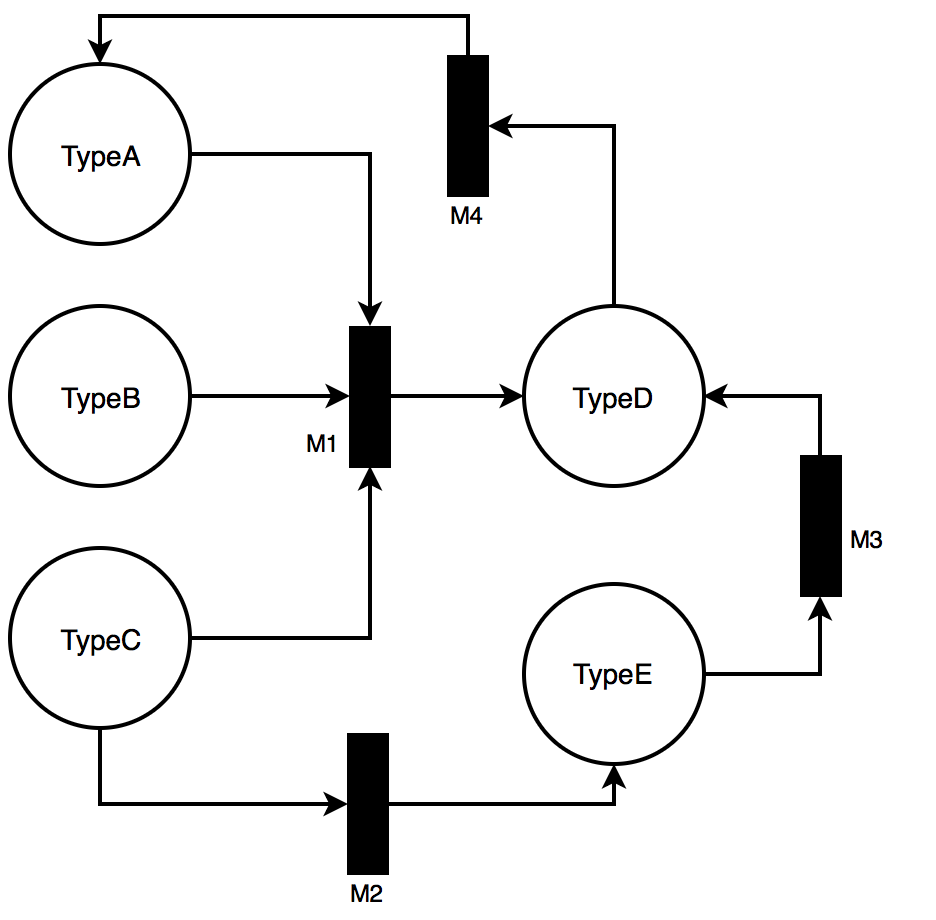
\includegraphics[scale = 0.35]{methoddemo.png}
\caption{Example network}
\end{figure}
The reachable path of the graph is defined as a subset of $A$ of all nodes in our network T. We find the set by modeling the problem as an SAT problem. A general procedural overview of our algorithm is shown in Figure 5.\\

\textbf{Variables}: for each of the n methods, we create a variable $m_i$, true if and only if the method is activated. For each of the k type, we create a variable $t_i$, true if and only if the type is activated. Define Input(i) be the number of inputs of type i.\\


\textbf{Constraint \#1}: each method requires all its input types all activated.\\
The corresponding SAT constraint: $$\forall i < n, m_i \rightarrow \bigwedge_{t_j \in in(m_i)} t_j$$

\textbf{Example}: for M1, $$M1 \rightarrow TypeA \wedge TypeB \wedge TypeC$$\\

\textbf{Constraint \#2}: each non-input type requires at least one method that generates this type to be activated.\\
The corresponding SAT constraint: $$\forall i < k, i \notin inputs, t_i \rightarrow \bigvee_{m_j \in in(t_i)} m_j$$
\textbf{Example}: for TypeD, $$TypeD \rightarrow M1 \vee M3$$

\textbf{Constraint \#3}: all input types and the return type should be activated. \\
The corresponding SAT constraint: $t_{return}$ true and $\forall t_i \in inputs, t_i$ true.\\

\textbf{Example}: If TypeD is our return type, then $$TypeD = 1$$


\textbf{Constraint \#4}: by our hypothesis, each return value should be used at least once. To make sure each return value is used at least once, for each type, the number of times of usage should be more than the number of variables generated of that type.\\
Specifically, $$\forall i < k, Input(i) + \sum_{m_j \in in(t_i)}m_j \leqslant \sum_{m_k \in out(t_i)}m_k$$ 

\textbf{Example}: for TypeE, $$M2 \leqslant M3$$

\textbf{Constraint \#5}: To guide our search, we start from programs of length 1, and increase the program length one at a time. To limit the length of our program, we add the length constraint:

For each program length k, $$\sum_{i=1}^{n} m_i = k$$

\textbf{Example}: at program length 3, $$M1+M2+M3+M4 = 3$$

With all these constraints, in most cases, we can guarantee that there exists at least one sequence of method calls such that we can find a compilable program, and there is no unused variable. Also, we ensure the as long as the Target program satisfies our hypothesis, we will eventually find the target program.\\ 

However, there are special cases, when the method calls form a loop, disconnected from the input types, in such a way that different types generate each other. This problem is handled by filtering the solution afterwards to ensure all activated types are reachable from the input paths with the activated path. The reachable path here is determined by a graph search algorithm such as BFS.\\


\section{Sketch generation and completion}
Given the set $A$, we can filter to find the set $B = A \cap M$ that correspond to the methods. Given set $B$, we determine possible orders of $B$. \\

We recursively generate possible permutations of set $B$ using the following algorithm by checking whether the type mapping pool can satisfy the input argument of methods:
\begin{algorithm}
\caption{Method Sequence Generator}\label{euclid}
\begin{algorithmic}
\State $S$: method set
\State $TM$: map from each type to the number of inputs
\Procedure{MSG($S,TM$):}{}
\Function{generator($S,TM$):}{}
\State $L=\{\}$
\For{$method$ in $S$}:
\State $args=method.inputArgTypes$
\State $TM'=fits(args,TM)$
\If{$TM'$ is $null$} \Return L \EndIf
\If{$s.returnType~\neq~"void"$}
\State $TM.get(s.returnType)$+=1
\EndIf
\State $S'=S/method$
\State $L'=\{method\}@$GENERATOR$(S',TM')$
\State $L=L+L'$
\EndFor
\State \Return $L$
\EndFunction
\Function{filter(L):}{}
\State \Return $\{S'\in L:|S'|=|S|\}$
\EndFunction
\Function{fits(args,TM):}{}
\For{$t$ in $args$}:
\If{$k \in TM.keys$}
\State $TM.get(k)$-=1
\Else
\State \Return $null$
\EndIf
\EndFor
\State \Return $TM$
\EndFunction
\State
\Return FILTER(GENERATOR(S,TM))
\EndProcedure
\end{algorithmic}
\end{algorithm}
\\
With set $B$ and type mapping $TM$, we use $MSG(B,TM)$ to acquire method call sequences. Given a sequence of method calls, we generate a program sketch by listing the method calls in order, leaving the specific variables empty. Consider the following sequence $<$getX(),getY(),new MyPoint(int,int)$>$ which takes in a Point object as input and returns a MyPoint object. Then, the corresponding sketch will be\\
\begin{figure}[h]
\centering
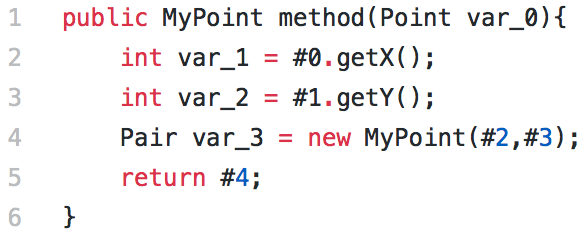
\includegraphics[scale = 0.7]{sketchcompeg.png}
\caption{An example program sketch}
\end{figure}\\
As for sketch completion, our goal is to determine which variables fit in each hole in the program. Our technique uses a SAT solver to find all possible programs.\\
Variables: $h_{i}^j$ if true if and only if $var_i$ goes to hole j.\\
Define $before(j)$ be all $i$ such that variable i is declared before hole j and has the same type as hole j. Define after(i) be all $j$ such that hole j appears after declaration of variable i and has the same type with variable i.\\

\textbf{Constraint 1}: there is a unique variable that goes to each hole
$$\forall j, \sum_{i \in before(j)}h_{ij} = 1$$
\textbf{Constraint 2}: each variable is used at least one once.
$$\forall i, \sum_{j \in after(j)}h_{ij} \geqslant 1$$

Once we have the code snippet of the program, we will compile and run the code generated by the synthesis tool, and run it against the test cases provided by the user. If a test cases passed, the program will return synthesized code as the solution. Otherwise, the synthesis tool will go back to the loop to look for other solutions.\\


\section{Equivalent program elimination}
We also explored an optimization technique that potentially improve the performance of our synthesis tool.
\begin{figure}[H]
\centering
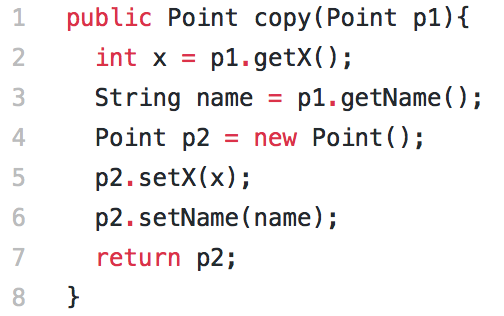
\includegraphics[scale = 0.7]{equiveg.png}
\caption{An example equivalent program}

\end{figure}\\
Consider the program in Figure 7. It's clear that line 2 and line 3 can be exchanged in order, and line 5 and line 6 can be exchanged in order, since the getX and getName are independent, and setX and setName are independent. To avoid equivalent programs to be explored multiple times, in this technique, we aim to determine dependency of methods, and use our definition to eliminate equivalent programs.\\

We determine whether methods are dependent by interprocedural analysis into the library code. We determine a set of non-local variables $P_i$ accessed by each method $m_i$. Then, two methods $m_i$ and $m_j$ can be exchanged in order if:
\begin{enumerate}
    \item $m_i$ and $m_j$ are consecutive in the target code.
    \item $P_i \cap P_j = \emptyset$
    \item $ret(m_j) \notin inputs(m_i)$ and $ret(m_i) \notin inputs(m_j)$
\end{enumerate}
Then we use a recursive process to find out all equivalent sequences of a sequence of method $S = \{m_{i1},m_{i2},...m_{is}\}$, where $|S| = s$, by exchange one consecutive pair at a time. Since the number of permutations is $s!$, the algorithm will guarantee to terminate. Also, since each permutation explored in the recursive process will correspond to a program eliminated, therefore saves compilation time, the equivalent program elimination process will not produce any performance overhead on the program.\\

\section{Implementation}
We have imlplmented the synthesis algorithm called SyChicken, consisting of approximately 5000 lines of Java code. SyChicken uses the Sat4j[1] tool for solving SAT problem, adn can be instantiated with any Java API to synthesis code with no conditional/loops. We only used Soot[2] to parse java libraries and perform interprocedural analysis for the libraries.\\

Note that since our implementation runs tests by recompiling the code snippet with the corresponding library, compilation is very time consuming compared to most of the other parts of the algorithm (SAT solving, network construction etc.). Therefore, we did not measure the total time of the program run, but broke the performance metrics into multiple parts, and measure each part independently.\\

\section{Evaluation}
To evaluate SyChicken, we performed experiments that were designed to answer the following questions:
\begin{enumerate}
    \item How well does SyChicken perform on component based synthesis tasks with Java APIs?
    \item How does SyChicken compare to SyPet, the existing tool for type-directed component based program synthesis?
    \item What is the effectiveness of equivalent program elimination in SyChicken?
\end{enumerate}
\subsection{Performance Metrics}
To answer the first and the second qeustions, we first create a metric to measure performance of SyChicken and SyPet.\\
We evaluate the performance of our algorithm by the performance metrics:
\begin{enumerate}
    \item Preprocessing time: time spent to build the network and set up the constraints.
    \item SAT solving time: time spent by the SAT solver.
    \item Percentage of valid set: as we mentioned before, some sets can correspond to no program due to the nature of our network. Therefore, we measure the percentage of sets that correspond to at least one program to show the effectiveness of our approach.
    \item The number of programs explored by the tool.
\end{enumerate}
\subsection{Results}
We created 11 benchmarks on the following libraries:
\begin{itemize}
    \item Point library (created): cmu.edu.Point
    \item Geometry library: java.awt.geom
    \item Math library: apache.commons.math
    \item Text and XML related libraries: jsoup, w3c.dom and javax.xml
\end{itemize}
Benchmarks typically aim for Target programs with 3-6 lines of code. Our measurements are shown in the provided table. We also performed the same measurements for SyPet.\\
\begin{figure}[h]
  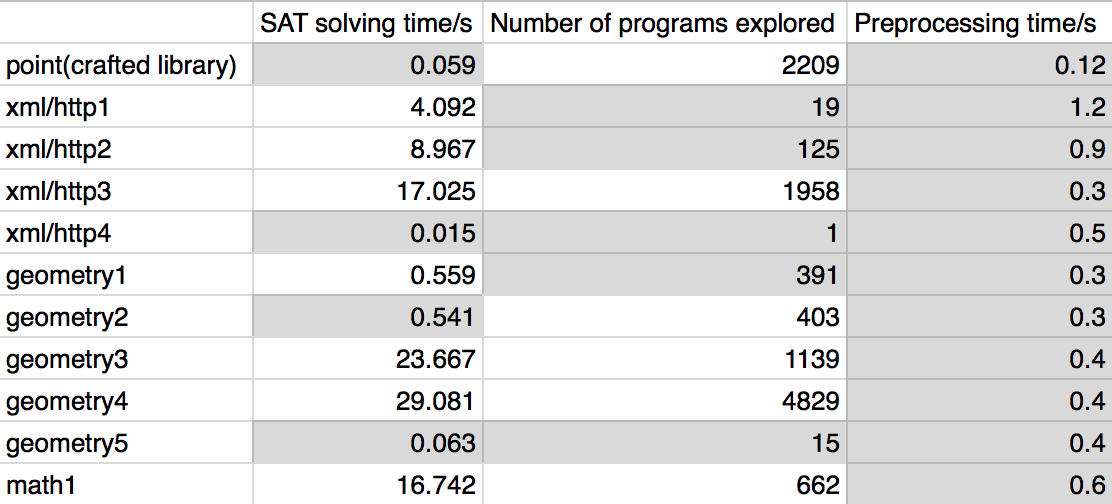
\includegraphics[width = \linewidth]{data1.png}
\caption{Summary of Experimental results of SyChicken (grey squares indicate SyChicken outperforms SyPet)}
\end{figure}\\
We can see from the data that SyChicken managed to synthesize 64\% of all programs within 10 seconds. (Note that we are excluding compilation time, since it creates a large overhead that independent to the benchmark itself.) In other cases, SyChicken explores more than 1000 reachable paths generated by the SAT-solver. We will discuss the performance overhead produced by our model in the next section.\\

\begin{figure}[h]
  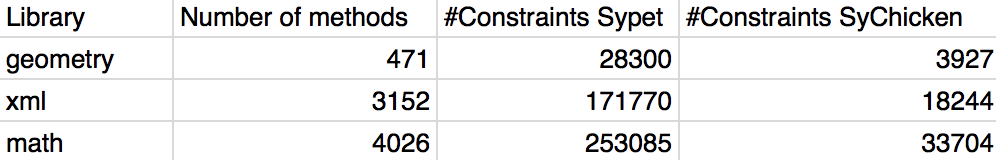
\includegraphics[width = \linewidth]{nconstr.png}
\caption{Number of SAT Solver Constraints in SyChicken is roughly 8 times smaller than in SyPet}
\end{figure}
Compared to SyPet, the performance of SyChicken is worse in major cases and better in some other cases in terms of set SAT solving time and number of programs explored. However, one huge advantage of SyChicken over SyPet is that the preprocessing time (including network construction and constraints setting) is extremely short with SyChicken usually below 1 second. In SyPet, building the network structure usually takes 10-30 seconds with geometry and math. Moreover, since in SyPet, all constraints will be reset as length increases, there is a repeated cost of setting constraints as the program length grow. By the comparison, though SyChicken performs worse than SyPet in terms of processing time, it is much more lightweight in terms of size of the encoding of the problem.

\subsection{Invalid paths}
\begin{figure}[h]
  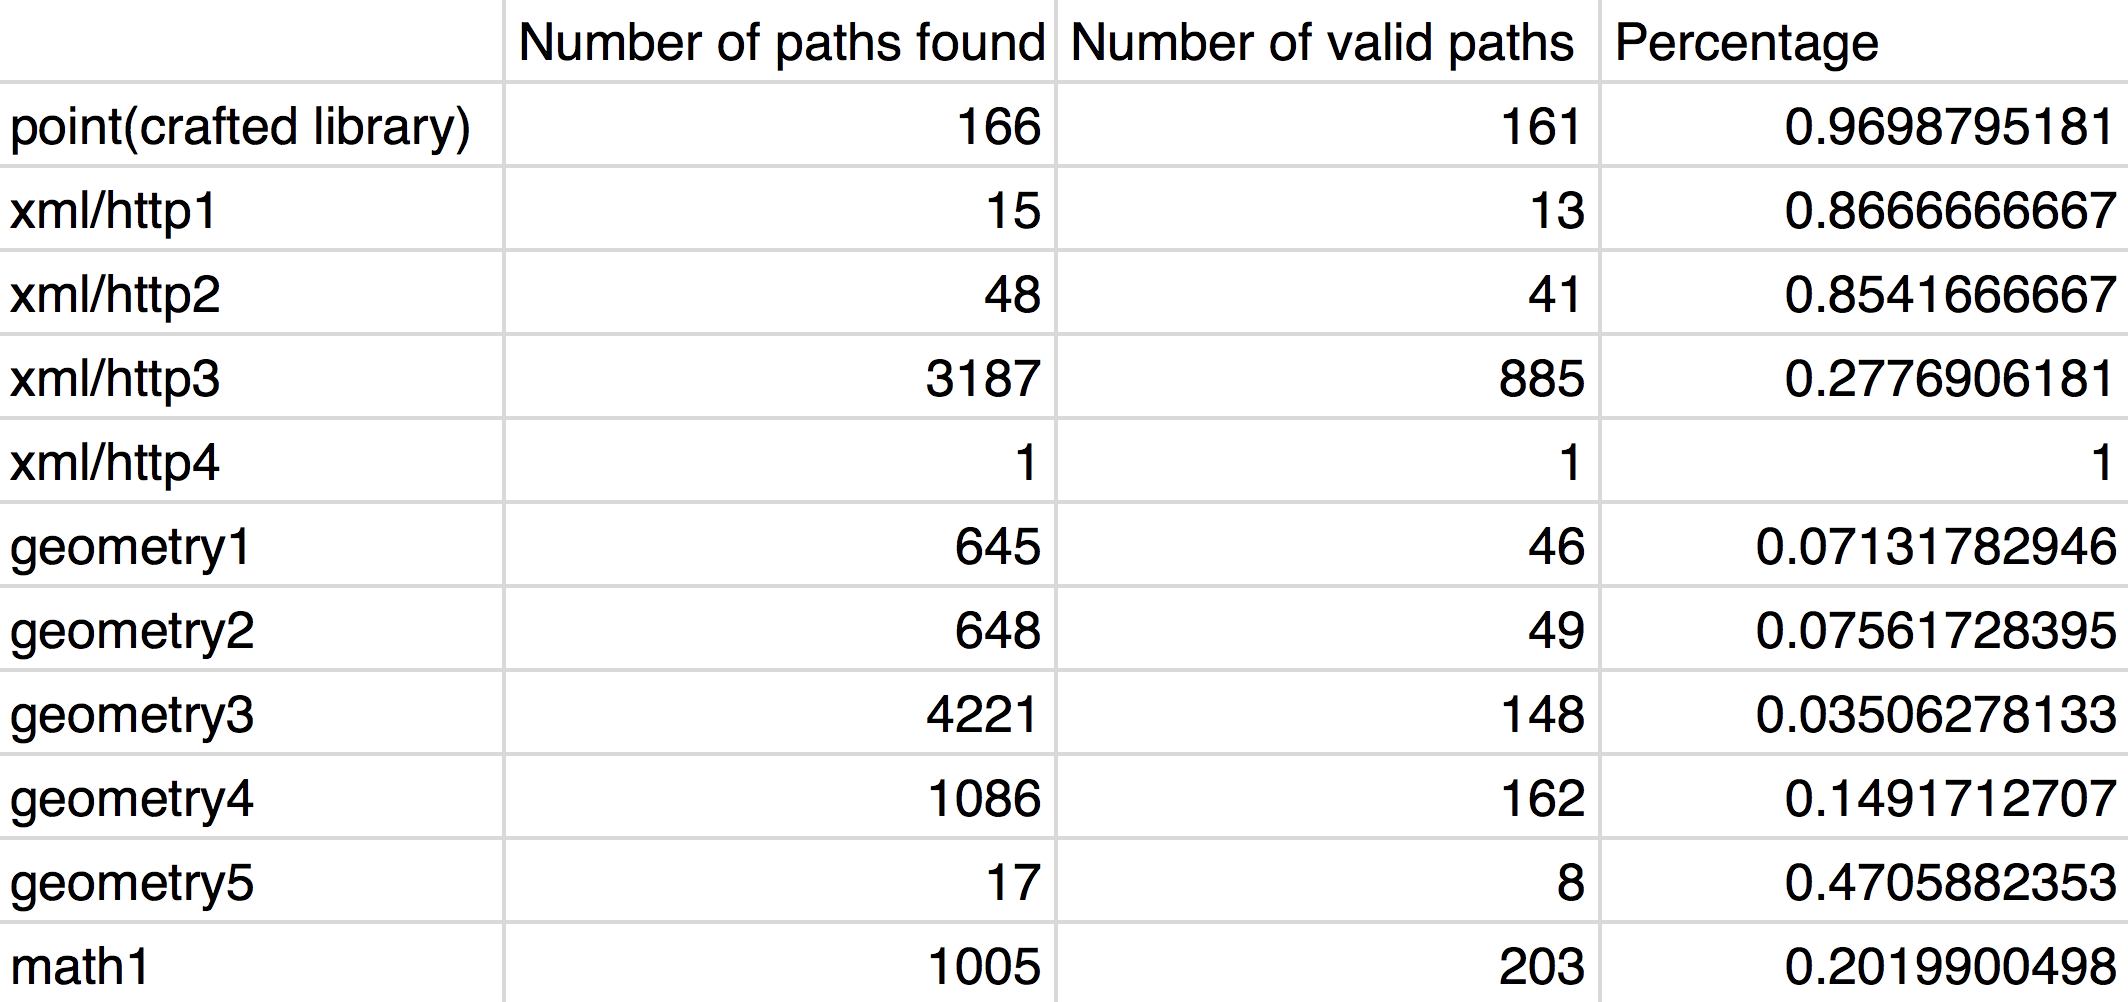
\includegraphics[width = \linewidth]{data2.png}
\caption{Summary of number of reachable paths explored by SyChicken}
\end{figure}
We measured for each benchmark, the number of reachable paths found by the reachability analysis using SAT solver before we reach the solution. We also measured the number of paths that correspond to at least one valid program that compiles and run.\\
As we can tell from the figure above, in some cases, typically in geometry 1,2 and 3, the percentage of valid paths is lower than 10\%, which means that at least 9 out of 10 paths found by SyChicken has no corresponding program. This can be explained as a consequence of the orderless property of our network. Since we have no notion of time, it is possible to generate types that does not really exist. For example, consider the 2 methods in figure.\\
\begin{figure}[h]
  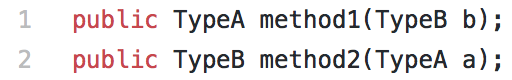
\includegraphics[width = \linewidth]{examplewrong.png}
\caption{Example methods}
\end{figure}
According to our constraints in reachability analysis, the 2 methods can appear in any program, regardless of what the input type or return type is, since they generate an instance of each other. However, in real program, method calls can only happen on distinct time steps. Therefore, such programs are not valid.\\

\subsection{Equivalent program elimination evaluation}
\begin{figure}[h]
  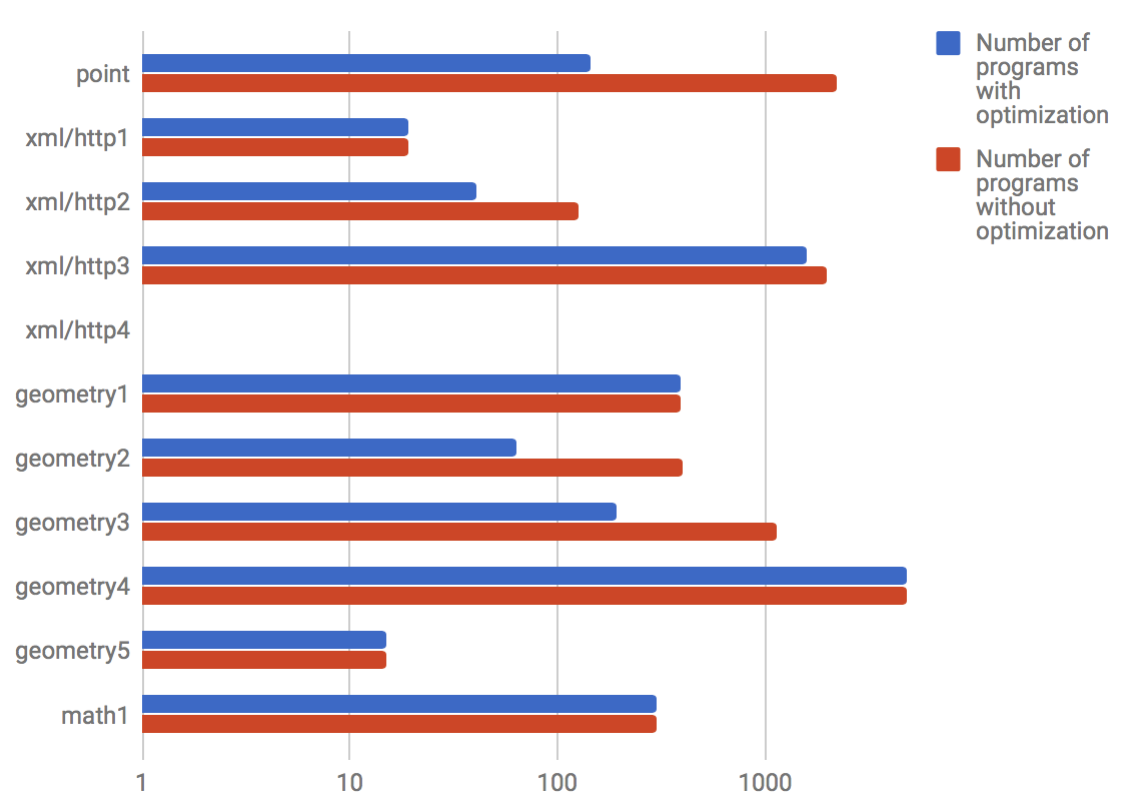
\includegraphics[width = \linewidth]{equivchart.png}
\caption{Effect of equivalent program elimination (on log scale)}
\end{figure}
We compared the performance of SyChicken before and after activating the program elimination, and obtained the data for each of the previous benchmarks.\\

It can be seen that according to our definition of equivalent programs, programs can be effectively eliminated in a domain where more methods are independent. For example, in Point library, more than 90\% of explored programs are eliminated. In other cases, for example in math and some examples in geometry, where methods are highly dependent, very few or no program can be eliminated.\\

\subsection{Recreate results}
To recreate results for the research, clone SyChicken from https://github.com/tpan496/SyChicken.git and see the instructions in README.md.
\section{Conclusion}
We have designed and implemented a new type-directed approach to component based program synthesis. Our approach builds a graph structure to model program components. Then we generate code sketches by analyzing reachable paths in the graph. The code sketches are then completed using SAT-based reasoning and tested on the user-provided examples.\\

After running all benchmarks, we found out even though that SyChicken did not outperform SyPet from SAT-solving time and number of programs explored, it does take significantly less time to build SyChicken's graph structure and SAT constraints due to the 8-9 times fewer number of constraints, and therefore SyChicken is more lightweight and flexible compared to SyPet.\\

We also explored and evaluated a technique that eliminates equivalent program based on interprocedural analysis into the provided libraries. Though the effect is not obvious in certain cases, the technique succeeds to eliminate 20\% of all programs on average.\\

\section*{Related Work}
 Another component-based synthesizer Prospector [4] utilizes the concept of a signature graph, which also adopts nodes and edges for types and methods, but does not have the concept of tokens. The user specifies a jungloid query that consists of a single input and output. Possible methods/edges (elementary jungloid) correspond to field access, static method/constructor invocation, instance method invocation, widening and downcast. The feasible paths (solution to the jungloid query) are then ranked according to length and returned to the user. According to the test results, Prospector is able to find the desired answer 18 out of 20 queries. However, the biggest drawback of Prospector is that it is limited to synthesizing methods that contain only single input/output.\\
 
 We have also looked into areas of machine learning, where models generated by machine learning are able to optimize the selection heuristics for program synthesis algorithms. One of the papers [5] purposes using k-nearest neighbors for auto-completion plugins in modern IDEs. The paper focuses on the java.swing package, where they use methods from swing library as labels. Each vector consists of 0 and 1 values that indicate whether a method appeared or not in the program of the training set. The prediction is based on given lines from the users, where they are used as constraints for rows and the prediction will be given in order of the frequency of labels appeared in the selected rows. Methods that have already appeared will be filtered out as they would have 1.0 probability under this model. The model was evaluated against a code base of 27000 user queries and is able to achieve an accuracy over 70 percent. One of the main drawbacks of this method is that it cannot deal with methods that may appear several times in a typical program; this drawback is also prevalent among most synthesis programs like SyPet and Prospector. Machine learning models may also be domain-specific, as the usage of some libraries can have a stronger structure for the sequence of calls than others do.\\


\section*{Acknowledgments}
We thank Ruben Martins for his insightful comments and providing information about SyPet.
We would also like to thank Claire Le Goues and Jonathan Aldrich for the knowledge provided about interprocedural analysis and program synthesis in 17-355 Program Analysis course.\\

\section*{References}
$[1]$ D.L. Berre and A. Parrain, The Sat4j library, release 2.2. Journal on Satisfiability, Boolean Modeling and Computation, pages 59-6, 2010.\\
$[2]$ R. Vallee-Rai, P. Co, E. Gagnon, L.J. Hendren, P.Lam, and V. Sundaressan. Soot-a Java bytecode optimization framework. In CASCON, page 13, 1999.\\
$[3]$ Y. Feng, R. Martins, Y. Wang, I. Dillig, T. W. Reps, Component-Based Synthesis for Complex APIs, POPL 2017\\
$[4]$ D. Mandelin, L. Xu, R. Bodik, Jungloid Mining: Helping to Navigate the API Jungle, 2005\\
$[5]$ M. Bruch, M. Monperrus, M. Mezini, Learning from Examples to Improve Code Completion Systems, 2007\\
$[6]$ SyChicken: https://github.com/tpan496/SyChicken.git.

\end{document}